\documentclass[12pt, a4paper]{article}
\usepackage[utf8]{inputenc}
\usepackage[T1]{fontenc}
\usepackage[french]{babel}
\usepackage{graphicx}
\usepackage{geometry}
\geometry{margin=2.5cm}
\usepackage{hyperref}
\usepackage{amsmath}
\usepackage{setspace}
\usepackage{float}
\usepackage{titlesec}

% Disable bold and italic in sections
\titleformat*{\section}{\Large}
\titleformat*{\subsection}{\large}
\titleformat*{\subsubsection}{\normalsize}

\onehalfspacing

\title{Rapport d'Analyse et de Conception : Exploitation des Donnees d'Accidents}
\author{DataValueXploring}
\date{\today}

\begin{document}

\maketitle
\tableofcontents
\newpage

\section{Presentation du role et de l'enjeu metier}

La prevention des risques routiers et l'optimisation des infrastructures de transport constituent des defis majeurs pour les collectivites territoriales. Dans le cadre de cette etude, nous incarnons le role d'une agence de voirie, couramment appelee Department of Transportation dans les pays anglo-saxons. Cette entite publique a pour responsabilite principale la gestion, l'entretien et l'amelioration continue du reseau routier sur un territoire donne. La securite des usagers est la priorite absolue de cette agence, qui doit composer avec des contraintes budgetaires souvent strictes et une infinite d'interventions possibles sur un reseau extremement etendu.

L'enjeu metier fondamental auquel nous sommes confrontes peut se resumer par la question suivante : comment reduire durablement le nombre et la gravite des accidents sur notre reseau, en optimisant l'allocation d'un budget de travaux limite ? Actuellement, la priorisation des travaux de voirie est frequemment reactive. Elle repond a des remontees du terrain, a des plaintes de citoyens, ou a la mediatisation de certains accidents tragiques. Bien que ces signaux soient importants, ils ne permettent pas de construire une strategie proactive, globale et rationnelle a l'echelle de tout un territoire. Une approche guidee par les donnees permet de depasser ce biais de mediatisation et de reactivite pour se concentrer sur le risque structurel reel.

Notre mission est de fournir une priorisation fondee sur des donnees tangibles, qui soit a la fois explicable aux elus et directement exploitable par les ingenieurs de la voirie. Le decideur public a besoin de reponses claires a des pragmatiques questions : ou doit-on intervenir en priorite absolue ? Et, une fois sur place, quel type d'equipement ou d'amenagement faut-il installer pour reduire le risque ? Notre role est donc de transformer un volume massif de donnees historiques d'accidents en un plan d'action prescriptif.

L'objectif final n'est pas simplement de dresser un constat des lieux les plus dangereux, mais d'identifier les leviers d'action infrastructurels. Les donnees utilisees proviennent du jeu de donnees US Accidents, couvrant la periode de fevrier deux mille seize a mars deux mille vingt-trois. Ce jeu de donnees contient pres de sept millions d'enregistrements d'accidents survenus dans quarante-neuf etats, avec un grand nombre de variables decrivant le contexte meteorologique, temporel et infrastructurel de chaque incident. L'exploitation de cette richesse d'informations nous permet de passer d'une gestion empirique a une gestion scientifique de la securite routiere.

Afin de repondre a cette commande, nous avons developpe un pipeline analytique qui part de la donnee brute et aboutit a des recommandations localisees. Le role de ce document est d'expliciter chaque etape de ce processus en demontrant comment l'approche choisie se justifie scientifiquement et produit de la valeur.

\section{Reformulation du probleme en termes de donnees et d'apprentissage automatique}

La problematique metier, bien que claire pour un decideur, n'est pas directement resoluble par un simple algorithme. Il est necessaire de la deconstruire et de la traduire en plusieurs taches specifiques d'analyse de donnees et d'apprentissage automatique. Nous avons choisi de scinder notre reponse en trois axes d'analyse correspondants aux trois questions fondamentales : Ou, Quoi et Quand. Chacune de ces dimensions appelle des outils methodologiques differents.

Le premier axe concerne le "Ou". La question est d'identifier les lieux qui concentrent le plus grand risque d'accidents graves. En termes de donnees, cela se traduit par une tache d'agregation geospatiale de grande ampleur. Il ne s'agit pas de predire le lieu du prochain accident de facon stochastique, mais de calculer une densite d'accidents historiques normalisee par le niveau de frequentation ou de densite du reseau routier. La traduction analytique consiste a discretiser l'espace geographique en cellules homogenes, a sommer les evenements par unite spatiale, et a diviser cette somme par un indice d'exposition. Le but est d'eviter un biais majeur : confondre les zones dangereuses avec les zones simplement tres frequentees ou le nombre d'accidents est eleve uniquement a cause de la loi des grands nombres.

Le deuxieme axe concerne le "Quoi". Une fois une zone dangereuse identifiee, il faut decider de l'amenagement a realiser. Faut-il ajouter un feu de signalisation, un panneau stop, un rond-point ? En apprentissage automatique, nous reformulons cette question comme un probleme de classification supervisee, mais utilise de maniere contre-intuitive. Au lieu de chercher a predire l'avenir, nous entrainons un modele a predire la gravite d'un accident historique a partir des caracteristiques de l'infrastructure et du contexte. L'objectif est d'utiliser le modele non comme un devin, mais comme un moteur de preuve. En interrogeant ce modele sur l'importance des variables d'infrastructure, nous identifions les elements qui aggravent ou atenuent la probabilite qu'un accident soit grave. C'est l'interpretation post-hoc du modele, basee sur des metriques d'explicabilite, qui fournit la prescription.

Le troisieme axe concerne le "Quand". Certains risques ne sont pas lies a des defauts d'infrastructure permanents, mais a des conditions meteorologiques specifiques ou a des periodes particulieres. La traduction en termes de donnees est une analyse descriptive et temporelle fine. Il s'agit d'identifier les patterns de gravite selon les heures de la journee, les jours de la semaine ou les conditions atmospheriques, afin de recommander des mesures temporaires, comme l'utilisation de panneaux a messages variables. Cette dimension est cruciale pour distinguer ce qui releve de l'amenagement permanent de ce qui releve de l'intervention ponctuelle.

Cette reformulation met en evidence que la performance predictive brute d'un algorithme (comme l'Accuracy ou l'Area Under the Curve) n'est pas la finalite de notre travail. Un modele avec une precision exceptionnelle mais totalement opaque (boite noire) ne serait d'aucune utilite pour notre agence de voirie, car il ne fournirait pas d'indications claires sur les actions a entreprendre sur l'infrastructure. Nous privilegions donc resolument des approches ou l'explicabilite et la quantification de l'effet causal potentiel des variables sont centrales. Le Machine Learning est ici un outil de decouverte de connaissances et d'evaluation de politiques, plutot qu'un simple generateur de previsions.

\section{Description detaillee de la demarche suivie}

Notre demarche suit un flux de travail rigoureux et systematique, allant de la preparation des donnees brutes jusqu'a la synthese decisionnelle presentee sous forme de tableaux de bord ou de listes de priorites. Chaque etape a ete concue pour garantir la reproductibilite de l'analyse sur n'importe quel sous-ensemble territorial du jeu de donnees. La qualite de la donnees initiale etant heterogene, une attention particuliere a ete portee aux phases de nettoyage et de pre-traitement.

\subsection{Collecte, nettoyage et fiabilisation des donnees}

La premiere etape a consiste a ingerer et traiter le volumineux jeu de donnees US Accidents. Les donnees issues de capteurs de trafic, d'applications de navigation ou de rapports de police sont par nature imparfaites, incompletes et parfois inconsistantes. Nous avons developpe un pipeline de nettoyage defensif. Ce nettoyage inclut la gestion rigoureuse des valeurs manquantes. Pour les variables meteorologiques telles que la temperature, l'humidite ou la visibilite, nous avons applique des methodes d'imputation basees sur la localite. Les enregistrements dont les coordonnees geographiques etaient aberrantes, manquantes ou situees en dehors des frontieres attendues ont ete systematiquement filtres et exclus de l'analyse.

Une decision cruciale a ete de redefinir et d'harmoniser les echelles de gravite. Le jeu de donnees propose une echelle de un a quatre, dependant fortement des criteres subjectifs des agences de signalement locales. Pour des raisons de prise de decision binaire pragmatique (doit-on financer une intervention urgente ou non ?), nous avons choisi de regrouper ces classes pour definir une variable cible binaire et robuste : accident grave contre accident non grave. Ce choix simplifie la modelisation tout en restant parfaitement aligne avec les priorites metier du departement de la voirie, qui cherche avant tout a reduire la mortalite et les blessures severes.

Ensuite, nous avons extrait et encode des variables temporelles pertinentes (heure de la journee, jour de la semaine, mois, jours feries) ainsi que des variables decrivant l'infrastructure au point GPS de l'accident (presence de ronds-points, de feux tricolores, de ralentisseurs, de passages a niveau). Ce travail d'ingenierie des caracteristiques est fondamental car c'est lui qui alimente le modele avec les variables actionnables par le decideur public.

\subsection{Analyse exploratoire temporelle et conjoncturelle (Le Quand)}

L'analyse exploratoire a d'abord porte sur les dimensions temporelles et meteorologiques. Nous voulions comprendre comment le risque evoluait independamment de l'infrastructure fixe, pour identifier les facteurs dits "conjoncturels" que l'amenagement urbain ne peut pas resoudre directement.

\begin{figure}[H]
\centering
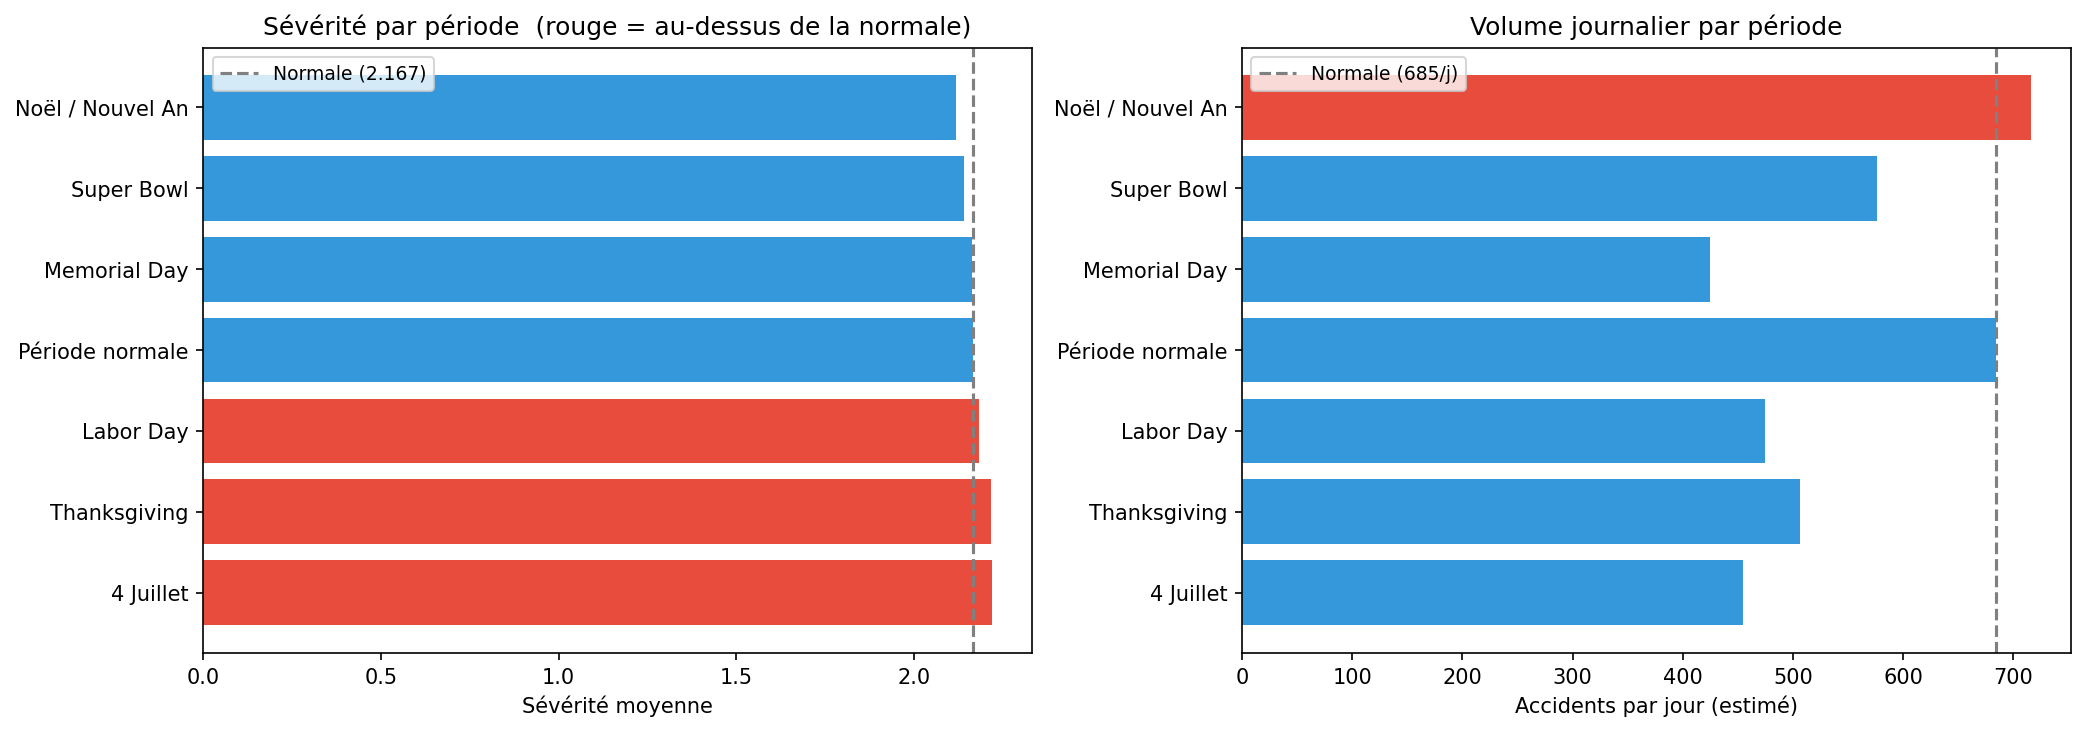
\includegraphics[width=0.8\textwidth]{../impact_evenements.png}
\caption{Impact des evenements temporels et de la meteo sur la proportion de gravite.}
\end{figure}

L'analyse visuelle et statistique de ces dimensions a mis en evidence des resultats parfois contre-intuitifs mais riches d'enseignements. Par exemple, la proportion d'accidents graves ne s'envole pas necessairement pendant les grands jours feries ou les fetes de fin d'annee, malgre une perception publique souvent contraire axee sur les comportements a risque durant ces periodes. De meme, l'analyse montre que les conditions meteorologiques tres degradees (brouillard epais, fortes pluies) forcent paradoxalement les conducteurs a adapter leur comportement et a reduire considerablement leur vitesse. Cela se traduit par une baisse significative de la proportion d'accidents graves, meme si le nombre absolu d'accrochages materiels peut augmenter.

A l'inverse, l'analyse par heure de la journee revele que les heures creuses (tard dans la nuit ou tres tot le matin) presentent des taux de gravite alarmants. La route deserte pardonne moins, car l'absence de trafic favorise des vitesses largement excessives qui transforment la moindre erreur de conduite en accident mortel.

Ces constats nous permettent d'ecarter les facteurs conjoncturels de notre priorisation infrastructurelle. Les problemes lies aux variations meteorologiques soudaines ou aux comportements specifiques de la nuit doivent etre geres par de la regulation de trafic dynamique (panneaux d'information, baisse limite de vitesse, eclairage), par des campagnes de prevention ou par des controles de police cibles, et non par des chantiers couteux de modification de voirie. Le budget de renovation, lui, doit se concentrer exclusivement sur le risque structurel.

\subsection{Identification des zones prioritaires (Le Ou)}

Pour determiner avec precision ou intervenir, il etait indispensable de discretiser l'espace geographique de maniere mathematiquement solide. Utiliser les limites administratives classiques (frontieres de villes, comtes, etats) est problematique car leurs tailles et formes varient enormement, ce qui fausse completement les densites calculees (effet d'unite spatiale modifiable). Nous avons choisi d'utiliser le systeme d'indexation spatiale hexagonale hierarchique (communement appele H3).

Ce systeme decoupe la surface de la terre en un pavage d'hexagones reguliers. En choisissant une resolution adaptee a l'enjeu urbain et periurbain, chaque hexagone represente une surface d'environ zero virgule sept kilometre carre. Cette granularite est ideale car elle correspond approximativement a l'echelle d'un grand complexe d'intersection, d'un rond-point majeur ou d'un troncon de boulevard significatif.

Pour chaque hexagone de la grille ainsi projetee sur le territoire, nous avons agrege le nombre total d'accidents historiques. Cependant, utiliser ce compte brut pour etablir un classement est profondement trompeur. Un carrefour situe en plein centre-ville affichera toujours un nombre d'accidents superieur a une intersection sur une route de campagne isolee, pour la simple raison mathematique qu'il voit passer un volume de vehicules cent fois plus important chaque jour.

Pour corriger ce biais d'exposition fondamental, nous avons integre massivement des donnees supplementaires provenant d'OpenStreetMap. Nous avons calcule la longueur totale et le type du reseau routier inclus dans chaque hexagone. L'indice de risque final, veritablement revelateur de la dangerosite intrinseque d'une zone, est calcule comme etant le nombre d'accidents divise par le kilometrage de voirie (et potentiellement pondere par le type de route).

Cette approche normalisee nous a permis de produire un classement reellement objectif et defendable des zones. Nous avons ainsi pu filtrer le territoire pour identifier les cinquante zones presentant le risque normalise le plus critique. Ces "points noirs", bien qu'ils ne representent qu'une fraction infime de la surface totale du territoire de l'etat, concentrent une part demesuree du fardeau accidentogene. Ce ciblage drastique est la premiere brique de la rationalisation budgetaire.

\subsection{Modelisation de la gravite et identification des leviers (Le Quoi)}

L'etape la plus complexe et novatrice de notre demarche a ete la modelisation. Pour les cinquante zones prioritaires prealablement identifiees comme dangereuses, nous devions aller au-dela du constat : nous devions savoir precisement quels equipements manquaient cruellement, ou a l'inverse, quels equipements inadaptes etaient associes a une surmortalite.

Pour ce faire, nous avons entraine plusieurs modeles de classification supervisee dont la tache etait de predire la variable cible binaire de gravite a partir des caracteristiques locales (presence d'un feu de signalisation, d'un passage pour pietons, d'un panneau d'arret, d'un ralentisseur), tout en forcant le modele a inclure et prendre en compte de nombreuses variables de controle (comme les conditions meteorologiques precises, la luminosite, l'heure de la journee et le type de route). L'inclusion de ces variables de controle est essentielle pour isoler mathematiquement l'effet "pur" de l'infrastructure.

Nous avons methodiquement compare une regression logistique lineaire et des modeles non-lineaires complexes comme les arbres de decision et les forets aleatoires. Une fois le meilleur modele selectionne et valide sur des donnees de test invisibles, sur la base de metriques adaptees aux donnees desequilibrees (comme la zone sous la courbe Precision-Rappel), nous avons altere sa fonction primaire. Au lieu de l'utiliser pour predire de nouveaux accidents (ce qui est inutile pour agir), nous l'avons utilise de maniere contrefactuelle via une methode d'inference causale appelee calcul-G.

Pour chaque accident present dans notre ensemble de donnees, nous avons demande au modele de predire la probabilite d'issue grave dans les conditions reelles. Ensuite, nous avons artificiellement et informatiquement modifie les donnees de cet accident specifique en changeant la presence d'un equipement (par exemple, en simulant l'ajout d'un panneau stop la ou il n'y en avait pas, tout en maintenant les conditions meteorologiques et horaires strictement identiques), et nous avons demande au modele de recalculer la nouvelle probabilite d'issue grave. La difference moyenne entre ces deux probabilites (reelle versus contrefactuelle) calculee sur un large echantillon nous donne l'effet ajuste de l'equipement. C'est cet effet ajuste, debarrasse de l'influence de l'environnement, qui dicte notre recommandation d'amenagement.

\section{Justification des choix methodologiques}

Chaque decision technique prise dans le cadre de ce projet ne resulte pas d'une preference arbitraire pour un algorithme a la mode, mais decoule directement des contraintes des donnees du monde reel et des besoins pragmatiques du decideur public. L'analyse de donnees ne se fait pas dans une tour d'ivoire, et les choix methodologiques doivent etre scientifiquement et fonctionnellement defensables face a un panel d'elus.

\subsection{Le choix de l'indexation hexagonale et de la normalisation de l'exposition}

L'utilisation du systeme de grille H3 se justifie mathematiquement par la necessite imperative d'avoir des unites d'analyse strictement homogenes et equidistantes. Contrairement aux grilles rectangulaires (latitude/longitude) qui souffrent de distorsions importantes aux poles et aux coins, le pavage en hexagones garantit que la distance entre le centre d'une cellule et les centres de toutes ses cellules voisines adjacentes est rigoureusement identique. Cette propriete topologique facilite grandement les calculs de voisinage spatiaux et assure une representation non biaisee du territoire lors des operations de regroupement.

L'integration fastidieuse des donnees d'OpenStreetMap pour calculer l'exposition kilometrique est un choix methodologique crucial, et represente un effort d'enrichissement de donnees majeur. Sans cette etape de normalisation, notre modele recommanderait invariablement au departement de la voirie d'analyser en boucle les grands boulevards peripheriques ou les nœuds autoroutiers les plus embouteilles. Certes, les accrochages (souvent a faible vitesse dans les bouchons) y sont innombrables, mais ils sont rarement graves. Pire, cette approche par compte brut conduirait a ignorer completement des routes secondaires moins frequentees, mais proportionnellement beaucoup plus letales en raison d'une configuration routiere dangereuse.

Le kilometrage lineaire de route extrait d'OpenStreetMap demeure un proxy imparfait pour le volume de trafic reel (Average Annual Daily Traffic), que nous ne possedons pas a une echelle nationale exhaustive. Cependant, c'est de loin le proxy le plus robuste, le moins sujet a des donnees manquantes asymetriques et le plus universellement disponible que nous pouvions utiliser pour garantir la reproductibilite de la methode sur n'importe quel etat nord-americain.

\begin{figure}[H]
\centering
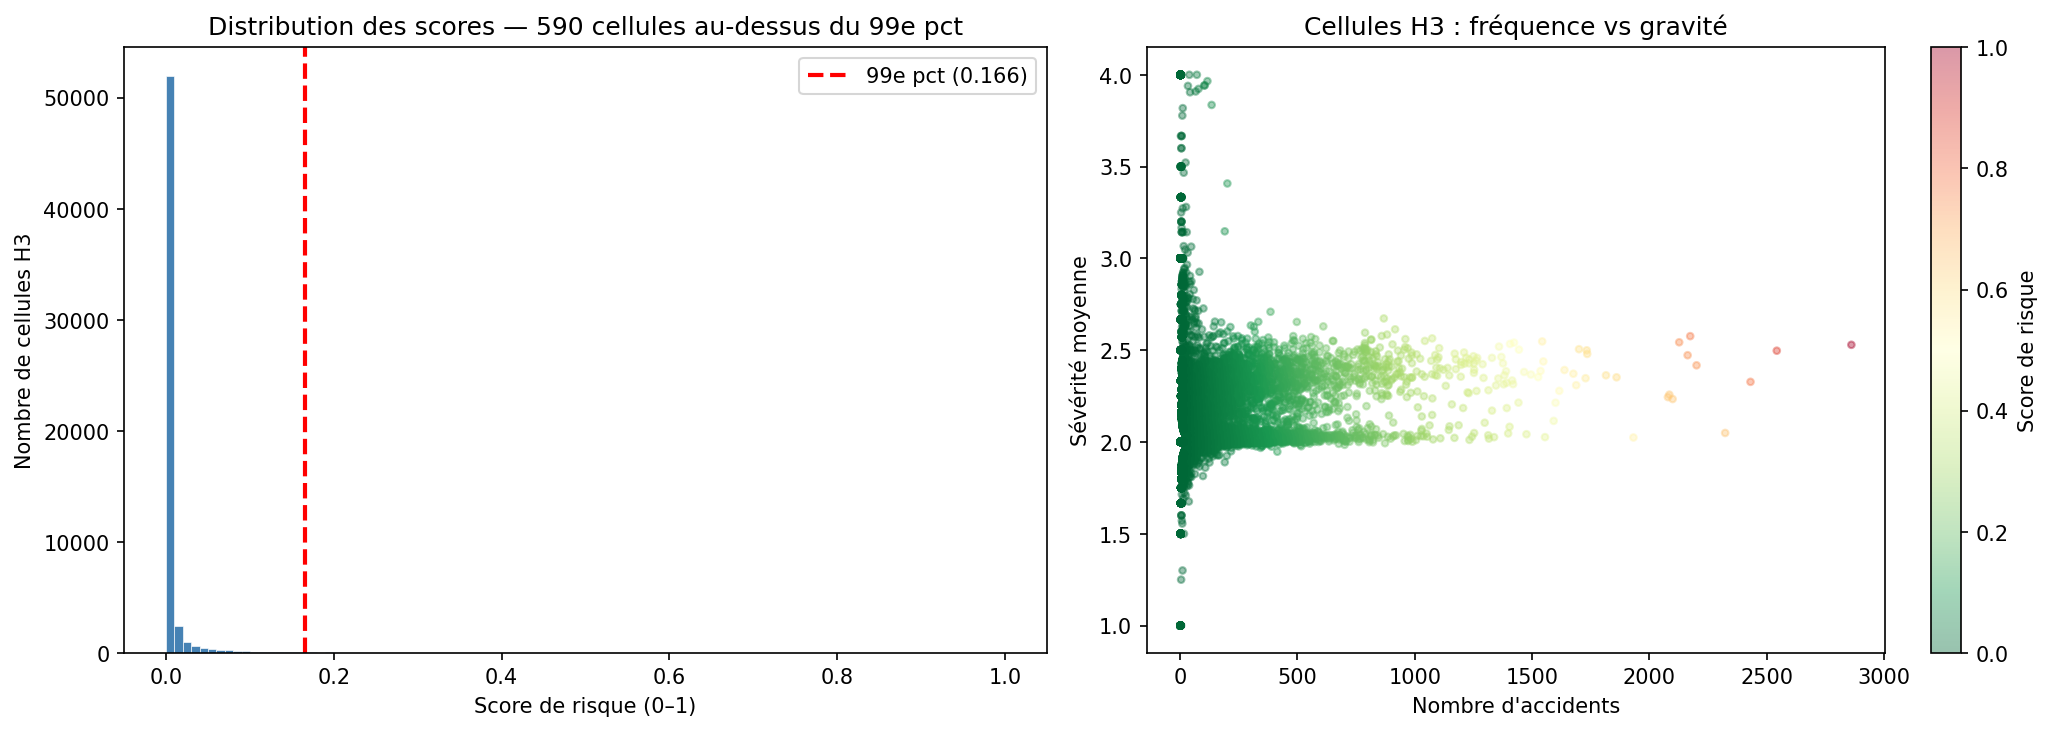
\includegraphics[width=0.8\textwidth]{../distribution_scores.png}
\caption{Distribution de la densite d'accidents : comparaison avant et apres l'etape de normalisation par le kilometrage OpenStreetMap.}
\end{figure}

La figure illustre a quel point la distribution des zones dangereuses change radicalement apres la normalisation. La normalisation ecroule les scores des zones tres etendues ou tres denses, et fait emerger les veritables points noirs : les zones ou le rapport entre le nombre de toles froissees et la quantite de route disponible est anormalement eleve.

\subsection{L'utilisation du modele d'apprentissage comme moteur d'explication}

L'apprentissage automatique (Machine Learning) est tres souvent enseigne et deploye industriellement comme une science de la prediction pure. Dans notre contexte metier specifique, la prediction pure est non seulement une impasse, mais aussi un risque. Un modele profond de type reseau de neurones ou un modele d'arbres complexes fonctionnant comme une boite noire parfaite, qui nous dirait avec quatre-vingt-dix-neuf pourcents de certitude que demain il y aura un accident grave a tel croisement precis a telle heure, ne nous aide pas le moins du monde a prevenir cet accident si le modele est incapable de nous dire de maniere intelligible pourquoi ce carrefour est dangereux.

C'est pour repondre a ce besoin absolu de prescriptivite que nous avons deliberement opte pour une demarche explicative post-modelisation. Le choix methodologique de commencer par une simple regression logistique et de la comparer a des modeles assembles (Random Forest) repond a un besoin fondamental de verification croisee et de robustesse.

La regression logistique offre une interpretation directe via l'analyse de ses coefficients, traduits en rapports de cotes (communement appeles odds ratios). Ces rapports indiquent de maniere explicite de combien la probabilite (ou plus precisement les cotes) d'avoir un accident grave est multipliee ou divisee en presence d'un element d'infrastructure donne.

Cependant, nous sommes conscients que la regression logistique impose une hypothese forte de linearite des effets, qui peut s'averer simpliste dans un environnement urbain complexe ou les interactions entre variables sont nombreuses. C'est pourquoi nous entrainons conjointement des modeles ensemblistes, reputes pour capturer ces non-linearites. Nous utilisons ensuite des techniques avancees d'explicabilite independantes du modele, comme les valeurs de Shapley, pour verifier rigoureusement si les relations lineaires et directionnelles decouvertes par la regression logistique tiennent toujours dans l'espace non-lineaire des forets aleatoires. Cette convergence des signaux (quand plusieurs modeles tres differents convergent vers la meme explication) est notre garantie de validite.

\subsection{La subtilite des valeurs d'explicabilite et les biais de confusion}

Lors de notre analyse et de l'interpretation des resultats des valeurs de Shapley, nous avons ete confrontes a un phenomene classique mais dangereux de confusion statistique (effet de variable confondante). L'analyse de l'effet global laissait entendre de maniere statistique que la presence de feux de signalisation et de passages pour pietons semblait augmenter la probabilite de gravite des accidents.

Si l'on appliquait aveuglement ces resultats (comme le ferait un systeme automatise non supervise), le systeme recommanderait au departement de la voirie de demonter et de supprimer les feux de circulation urbains, ce qui serait evidemment absurde, ethologiquement indigne et hautement dangereux.

Cette anomalie statistique apparente s'explique par le fait que les feux tricolores et les passages pietons ne sont pas installes aleatoirement sur le territoire. Ils sont systematiquement places dans des zones urbaines particulierement denses, aux intersections les plus complexes et les plus frequentees. C'est precisement dans ces zones que le risque intrinseque d'accident, impliquant souvent des vehicules legers, des cyclistes et des pietons, est mecaniquement plus eleve a cause des nombreux conflits d'usage de l'espace. L'equipement signale la presence du danger et tente de le reguler, il ne le cree pas.

C'est la raison fondamentale pour laquelle nous n'utilisons jamais les effets globaux ou les valeurs d'importance brutes pour prendre des decisions d'infrastructure. Pour contourner ce biais de selection, nous calculons des effets ajustes conditionnels. Nous mesurons mathematiquement l'effet d'un amenagement donne (via la technique du calcul-G evoquee precedemment) uniquement dans des sous-ensembles de zones presentant exactement le meme niveau d'alea local et de complexite. Cette stratification permet de neutraliser le facteur de confusion lie a la densite urbaine et de reveler l'effet protecteur reel des equipements.

\subsection{La validation empirique de la stabilite temporelle du risque}

Un defi majeur pour une agence d'amenagement urbain est de s'assurer que les lourds travaux d'infrastructure entrepris, dont la planification et l'execution prennent des annees, auront un impact durable a tres long terme. Si notre algorithme classe une zone geographique comme extremement dangereuse une annee donnee uniquement a cause d'un chantier de construction temporaire, de la deviation ponctuelle d'un flux de trafic, ou pire, d'une simple anomalie statistique ephemere, inciter la collectivite a investir massivement pour modifier l'infrastructure de maniere permanente constituerait un colossal gaspillage de fonds publics.

\begin{figure}[H]
\centering
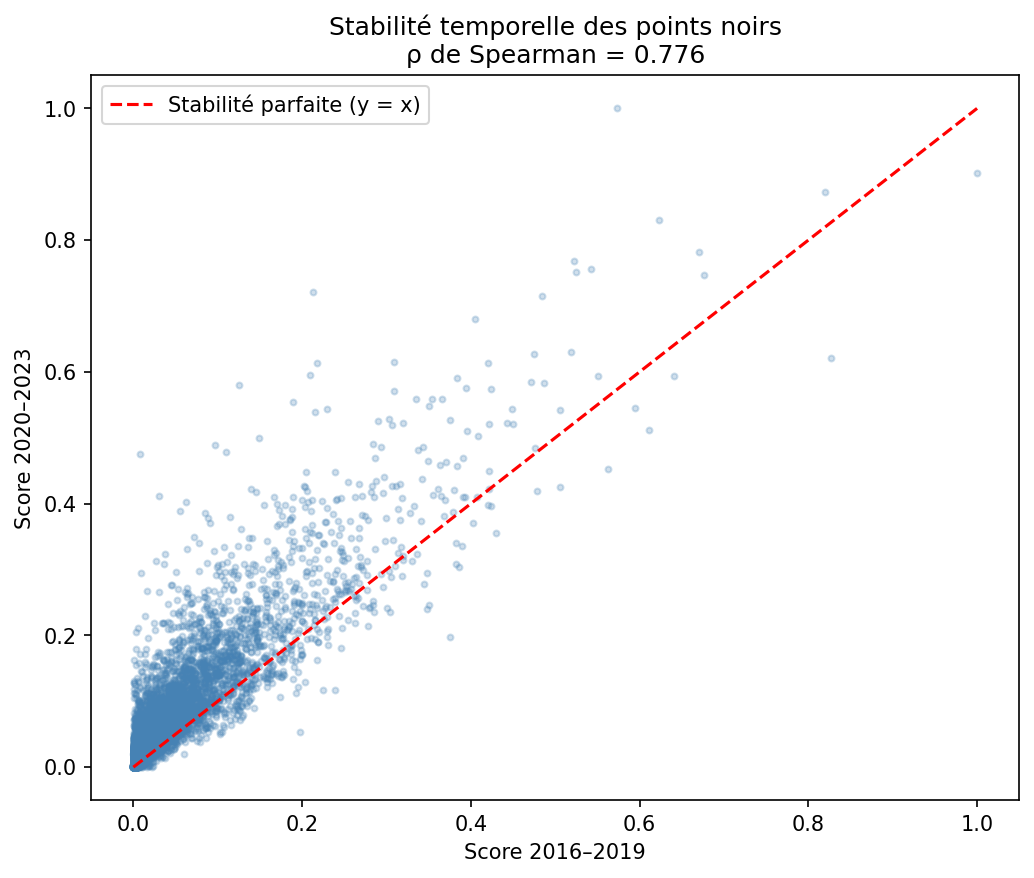
\includegraphics[width=0.8\textwidth]{../validation_stabilite.png}
\caption{Analyse empirique et validation de la stabilite temporelle des cinquante zones prioritaires (points noirs) a travers deux periodes distinctes.}
\end{figure}

Pour valider la solidite de notre approche et garantir que nous capturons bien un risque structurel, nous avons mis en place un protocole de validation temporelle strict. Nous avons scinde sciemment nos donnees historiques globales en deux periodes chronologiques completement distinctes (par exemple, la periode allant de fevrier deux mille seize a la fin de l'annee deux mille dix-neuf d'une part, et la periode de l'annee deux mille vingt a mars deux mille vingt-trois d'autre part).

Nous avons ensuite reexecute l'integralite de notre pipeline de scoring geographique (calcul des densites et normalisation par l'exposition) de maniere strictement independante sur ces deux periodes. L'objectif etait de verifier la correlation des rangs (en utilisant des metriques non parametriques comme le coefficient de correlation de rang de Spearman) des cinquante zones declarees les plus dangereuses entre la premiere et la seconde periode.

Les resultats de cette validation, illustres par la figure ci-dessus, demontrent une correlation tres elevee et une stabilite frappante. Les zones prioritaires identifiees ne resultent en aucun cas d'un bruit statistique erratique ; elles representent un dysfonctionnement structurel majeur et persistant du reseau routier. Ce constat apporte la garantie scientifique indispensable au decideur politique pour justifier un investissement dans des infrastructures physiques perennes sur ces lieux precis.

\section{Explicitation de la valeur creee et des limites de l'approche}

Le travail d'analyse de donnees developpe tout au long de cette etude ne prend son veritable sens que lorsqu'il depasse le cadre academique ou exploratoire pour etre traduit en valeur actionnable, mesurable et appropriable par l'utilisateur final metier. Il est par ailleurs indispensable, d'un point de vue ethiquement et scientifiquement responsable, d'en expliciter les limites methodologiques de maniere totalement transparente. Ne pas reconnaitre les angles morts d'un modele d'apprentissage automatique est la voie la plus courte vers la mise en echec de son deploiement.

\subsection{Creation de valeur pour la prise de decision strategique et operationnelle}

La valeur principale et immediate de notre solution analytique reside dans sa capacite a objectiver, racionaliser et pacifier les debats, souvent politiques et passionnes, autour de l'allocation des budgets de securite routiere. Le departement de la voirie ne navigue plus a vue ; il dispose desormais d'un outil quantitatif, auditables et entierement reproductible qui genere, a frequence reguliere, une liste decroissante de zones geographiques a traiter en absolue priorite.

Cependant, la solution proposee va beaucoup plus loin qu'un simple palmares des routes les plus meurtrieres. Pour chaque zone identifiee dans le peloton de tete (les points noirs), l'outil croise l'alea local caracteristique de cette zone avec l'effet ajuste conditionnel des differentes mesures protectrices qui y sont actuellement absentes.

Le resultat de ce croisement n'est plus une donnee statistique abstraite, mais une recommandation d'amenagement specifique, directement lisible par un ingenieur. Par exemple, si l'outil analyse la zone prioritaire numero cinq, identifiee comme etant un grand carrefour presentant un fort historique d'accrochages et de collisions laterales, il est capable de recommander l'etude prioritaire pour l'installation d'une signalisation avancee ou d'un stop. Il justifie cette recommandation en montrant que le modele estime que cette intervention a un impact conditionnel negatif significatif sur la probabilite de gravite dans ce type precis de contexte routier, et ce, toutes choses etant egales par ailleurs concernant la meteo ou l'eclairage.

Mieux encore, cette recommandation technique est assortie d'une estimation quantitative ex-ante de l'impact social attendu. En multipliant l'effet ajuste attribue a la mesure par le volume historique d'accidents pertinents observes dans la zone, le pipeline analytique fournit un chiffre estimatif precis du nombre d'accidents graves qui pourraient raisonnablement etre evites. Ce chiffre, meme s'il demeure une approximation statistique ex-ante, constitue un argument decisif. Il permet aux ingenieurs et aux decideurs politiques de realiser de veritables analyses cout-benefice avant de defendre ou de voter les budgets d'amenagement lourds lors des conseils municipaux ou regionaux. La valeur est donc double : technique (quoi faire) et politique (combien de vies sauvees pour quel budget).

\subsection{Limites inherentes aux sources de donnees et au processus de modelisation}

Nous assumons pleinement plusieurs limites contraignantes dans cette etude, qui delimitent le perimetre de confiance que l'on peut accorder aux recommandations.

La premiere limite, et de loin la plus fondamentale sur le plan epistemologique, est l'absence de causalite formelle mathematiquement demontree. Toutes nos recommandations, aussi robustes soient-elles, demeurent basees sur des associations statistiques ajustees, et en aucun cas sur des experiences controlees randomisees. Le jeu de donnees historique ne contient pas l'information longitudinale cruciale de la date d'installation des equipements sur le terrain. Nous ne pouvons donc pas observer dynamiquement le meme carrefour avant et apres l'ajout d'un feu de signalisation ou la construction d'un rond-point. Nous sommes reduits a comparer transversalement des carrefours equipes a des carrefours non equipes a un instant donne. Malgre tous nos efforts pour inclure des variables de controle, des variables confondantes non observees ou non mesurees (comme la qualite du revetement, l'angle de visibilite, la presence de vegetation ou la signalisation horizontale effacee) peuvent persister et biaiser partiellement les estimations d'impact.

La deuxieme limite majeure a trait aux facteurs humains, deliberement ecules par l'approche infrastructurelle. La litterature en accidentologie rappelle qu'un accident de la route est quasi-systematiquement la conjonction tragique d'une infrastructure defaillante et d'une erreur humaine. Or, notre modele predictif est completement aveugle a cette seconde composante. Il ne possede strictement aucune information sur l'age du conducteur, son etat de fatigue, son eventuel taux d'alcoolemie, ou surtout, sa vitesse d'impact reelle par rapport a la limite autorisee. Par consequent, le pouvoir predictif global intrinseque du modele (sa capacite absolue a predire la gravite de chaque accident) restera systematiquement plafonne et modere. L'infrastructure, meme parfaite, ne peut pas tout expliquer et ne saurait tout prevenir. Nous avons par ailleurs observe que sur une certaine proportion de zones tres accidentogenes, le modele echoue a identifier un quelconque levier d'amenagement pertinent. Cette impuissance apparente de l'outil n'est pas un echec, mais un resultat en soi : elle signale de maniere forte que la racine du probleme dans ces zones releve tres probablement du comportement des usagers. L'action requise n'est alors pas du ressort de l'ingenierie civile de la voirie, mais appelle a des campagnes de sensibilisation, une augmentation des controles radars ou des interventions policieres.

Enfin, il faut absolument souligner un biais structurel lie au processus de remontee des donnees lui-meme. Les informations agrenees par les fournisseurs de services de trafic et les applications de navigation grand public ont une propension naturelle a sur-representer massivement les incidents survenus sur les grands axes autoroutiers, les routes nationales et les voies urbaines denses. Inversement, elles peuvent sous-declarer les accrochages mineurs survenus sur des routes rurales isolees ou dans des zones residentielles a tres faible connectivite reseau, faussant potentiellement l'exhaustivite de notre carte theorique des risques a l'echelle du territoire. L'outil reste tributaire de la qualite de son alimentation.

\subsection{Perspectives d'evaluation empirique sur le terrain}

Pour pallier l'absence structurelle de preuves causales irrefutables dans les donnees historiques retrospectives, et pour assoir definitivement la legitimite du systeme, la valeur theorique de cet outil d'aide a la decision doit imperativement se concretiser par une evaluation empirique et rigoureuse sur le terrain.

Nous recommandons vivement au decideur public de ne pas utiliser l'outil pour justifier un deploiement d'amenagements a l'echelle de la totalite de l'etat de maniere precipitee. La demarche la plus scientifiquement saine consiste a utiliser les resultats du modele pour selectionner un petit groupe de zones pilotes, restreint et tres controle, comprenant par exemple dix intersections ou troncons classes dans les plus hautes priorites.

Sur ce groupe de dix zones traitees, les amenagements prescrits par le modele seront financierement programmes et physiquement realises. En parallele, un groupe de controle compose de dix autres zones presentant des scores de risque initiaux tout a fait similaires et des configurations infrastructurelles comparables ne recevra absolument aucun amenagement dans un premier temps. En instaurant un suivi sur une duree d'au minimum un an ou deux, et en mesurant precisement la difference de l'evolution du nombre d'accidents graves entre le groupe traite et le groupe de controle, la methode econometrique dite des doubles differences (Difference-in-Differences) permettra de quantifier de facon incontestable le veritable impact causal des travaux engages.

C'est seulement a l'issue de cette experimentation grandeur nature que l'estimation ex-ante du nombre d'accidents evites, theoriquement calculee par notre algorithme de Machine Learning, pourra etre confrontee a l'epreuve de la realite du terrain et de la circulation reelle, validant ainsi definitivement la chaine de valeur proposee par cette demarche axee sur les donnees.

\section{Conclusion}

Ce projet extensif demontre de maniere eclatante comment des gisements de donnees massives, souvent imparfaites et heterogenes, peuvent etre transformes methodiquement en un veritable levier d'action publique et de pilotage strategique. En refusant fermement la vacuite intellectuelle et operationnelle d'une prediction en boite noire, et en imposant au contraire au modele d'apprentissage automatique de justifier ses liens avec l'infrastructure de facon interpretable, nous avons reussi a concevoir un processus decisionnel transparent et defendable.

L'agence de voirie territoriale dispose desormais grace a ce travail d'un protocole complet, reproductible et end-to-end, allant de l'identification geographique objective d'un danger chronique jusqu'a l'estimation quantitative a priori de l'impact social d'une renovation ciblee. Bien que ce systeme automatise n'ait pas vocation a remplacer le jugement qualitatif, la connaissance locale ni l'expertise humaine fondamentale des ingenieurs sur le terrain, il rationalise considerablement le processus en amont. Il oriente les precieux budgets d'amenagement la ou l'impact potentiel sur la securite publique est statistiquement le plus grand, et fournit une argumentation rationnelle et basee sur des preuves mathematiques pour la gestion de la securite routiere, elevant ainsi le niveau de service rendu aux citoyens et usagers de la route.

\end{document}
